Analysis of the top 10 trigrams showed patterns like ``wed number aug'', ``number aug number'', ``date number number'', suggesting frequent date/number sequences or mailing list headers (list listinfo mail).
These patterns might help identify specific email types.

\begin{figure}[H]
    \centering
    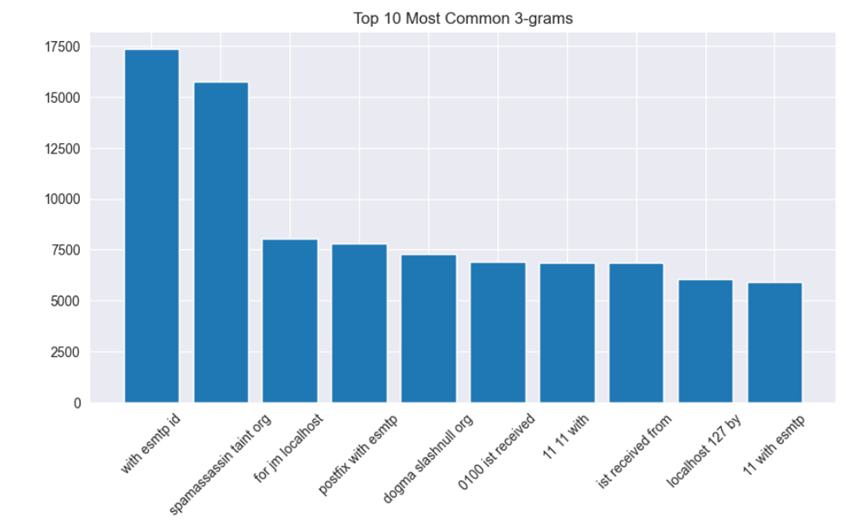
\includegraphics[width=\linewidth]{images/common_tri_grams}
    \caption{Bar Chart for 10 Most Common Trigrams}
    \label{fig:common_tri_grams}
\end{figure}

Observations:
\begin{itemize}
    \item The trigram ``with esmtp id'' is the most frequent, appearing significantly more often than the others.
    \item The trigram ``spamassassin taint org'' is the second most frequent.
    \item The remaining trigrams have lower and relatively similar frequencies.
    \item The trigrams suggest that the email data contains technical information, likely related to email headers and processing (``esmtp'', ``localhost'', ``received'') and spam filtering (``spamassassin'', ``taint'').
\end{itemize}

Potential Meaning:
\begin{itemize}
    \item The most frequent trigrams indicate the common occurrence of information related to email headers and the email transmission process.
    Phrases like ``with esmtp id'', ``postfix with esmtp'', ``ist received'', ``received from'', and ``localhost 127 by'' all pertain to how emails are sent and received.
    \item The presence of ``spamassassin taint org'' suggests that spam filtering activity is a significant aspect of this dataset.
    \item Other trigrams like ``for jm local/host'', ``dogma slashnull org'', ``0100 ist received'', ``11 11 with'', and ``11 with esmtp'' might relate to specific systems, software, or characteristic data formats within the context of this dataset.
\end{itemize}

Conclusion:

This chart reveals that information related to email processing and headers, as well as spam filtering activities, are prominent features in the analyzed text dataset.
The other trigrams may provide further insights into specific systems or formats relevant to this data.